\documentclass[10pt]{article}
\usepackage[margin=1in]{geometry}
\usepackage{amsmath,amssymb}
\usepackage{booktabs}
\usepackage{graphicx}
\usepackage{microtype}
\usepackage{xcolor}
\usepackage{hyperref}
\hypersetup{colorlinks=true,linkcolor=blue,urlcolor=blue,citecolor=blue}
\graphicspath{{./}}
% Auto-generated by studies/next_stage_validation/scripts/render_paper_artifacts.py
\newcommand{\AgentSeedCount}{3}
\newcommand{\AgentEpisodes}{128}
\newcommand{\MeanNeuralAdaptive}{-0.022}
\newcommand{\ObsConstrainedCoverage}{0.790}
\newcommand{\ObsConstrainedWrong}{0.075}
\newcommand{\ObsConstrainedUnresolved}{0.905}
\newcommand{\InterventionNoneRate}{0.090}
\newcommand{\InterventionThrottleRate}{0.000}
\newcommand{\InterventionThrottleDrawdown}{0.010}
\newcommand{\AgentResultsTable}{%
\begin{tabular}{lrrrr}
Seed & No trade & Adaptive & Neural & Neural - adaptive\\\hline
601 & 0.000 & -0.093 & -0.183 & -0.090\\
602 & 0.000 & -0.093 & -0.116 & -0.023\\
603 & 0.000 & -0.093 & -0.045 & 0.048\\
\end{tabular}%
}
\newcommand{\ObservationResultsTable}{%
\begin{tabular}{lrrrr}
Condition & Coverage & Decisive & Wrong confident & Unresolved\\\hline
exact\_independent & 1.000 & 1.000 & 0.000 & 0.000\\
noisy\_independent & 0.835 & 1.000 & 0.000 & 0.000\\
noisy\_dependent & 0.795 & 1.000 & 0.000 & 0.000\\
noisy\_dependent\_missing & 0.805 & 1.000 & 0.000 & 0.000\\
constrained\_noisy\_dependent & 0.790 & 0.095 & 0.075 & 0.905\\
\end{tabular}%
}
\newcommand{\InterventionResultsTable}{%
\begin{tabular}{lrrr}
Policy & Event rate & Gain & Drawdown\\\hline
none & 0.090 & -0.939 & 0.023\\
throttle & 0.000 & -0.387 & 0.010\\
liquidate & 0.043 & -0.838 & 0.021\\
\end{tabular}%
}
\newcommand{\CalibrationResultsTable}{%
\begin{tabular}{lrrrr}
Asset & Train & Validation & Test & Return volatility\\\hline
BTCUSDT-1m-2025-01 & 26784 & 8928 & 8928 & 0.00080\\
ETHUSDT-1h-2025-01 & 446 & 148 & 150 & 0.00734\\
SOLUSDT-1h-2025-01 & 446 & 148 & 150 & 0.01238\\
\end{tabular}%
}
\newcommand{\LTwoCalibrationTable}{%
\begin{tabular}{lrrrrr}
Symbol & Test days & Snapshots/day & Trades & Flow ACF & Return vol.\\\hline
BTCUSDT & 7 & 2880 & 10725827 & 0.521 & 0.00003\\
ETHUSDT & 7 & 2880 & 11111798 & 0.561 & 0.00003\\
SOLUSDT & 7 & 2880 & 3443026 & 0.257 & 0.00006\\
\end{tabular}%
}


\title{What Offline Observations Can Establish About Adaptive Feedback in Machine Markets}
\author{Machine Markets project\\\small Authorship and contribution review pending}
\date{18 September 2026}

\newcommand{\codelink}[1]{\texttt{#1}}

\begin{document}
\maketitle

\begin{abstract}
We report a reproducible next-stage validation of a machine-markets research
release. The study separates measurement uncertainty, adaptive-policy
comparisons, and operational loss. In an independently specified synthetic
market, a small neural policy was trained by deterministic population search and
compared on paired held-out tapes with a fixed no-trade rule and a hand-written
adaptive non-neural controller. Across three training seeds and 128 held-out
episodes per seed, the mean neural-minus-adaptive gain was
\MeanNeuralAdaptive{} account units, far below the predeclared 0.5-unit effect
threshold; no AI-specific advantage is supported. A separate observation
benchmark shows that a constrained noisy/dependent condition had 0.790 interval
coverage, 0.075 wrong-confident calls, and 0.905 unresolved calls. In a
difficult synthetic risk regime, a 50\% execution throttle reduced the
nonterminal event rate from \InterventionNoneRate{} to
\InterventionThrottleRate{} while reducing mean drawdown to
\InterventionThrottleDrawdown{}. These are controlled synthetic findings, not
real-market probabilities or safety guarantees. Public Binance OHLCV data are
used only for a chronological descriptive pilot; full order-book calibration,
external replication, and independent publication review remain open.
\end{abstract}

\section{Scope and research question}

The central question is deliberately narrower than the original ambition:
what can observations and declared architectural information establish about
adaptive feedback at a stated economic cost, and what remains necessary to
assess operational loss? We distinguish three targets that are often conflated:
local signal stability, finite-observation inference, and financially induced
loss or halt events. A numerical test of one target is not evidence for the
others.

This paper is a new evidence layer on top of the frozen Machine Markets release.
The four historical study packages and their checksums are preserved. New code
is under \codelink{studies/next\_stage\_validation/}; its outputs are not pooled
with the original synthetic denominators.

\section{Information contract and environment}

The new environment is a separate CPU-only implementation with explicit price,
cash, inventory, spread, depth, impact, partial fill, fee, margin, drawdown, and
halt logic. At each step an agent observes a seven-component public vector:
price return, normalized inventory, equity change, spread, depth, margin ratio,
and normalized time. Shock values and future prices are not exposed. The action
is a requested signed quantity in $[-1,1]$.

The primary confirmation configuration uses a 48-step horizon, 100 units of
initial cash, maximum order 0.5, maximum inventory 2, spread 0.02, depth 5,
impact 0.04, volatility 0.01, fee rate 0.001, and partial-fill parameter 0.15.
The environment is a controlled synthetic mechanism, not a claim to reproduce
an exchange.

\section{Matched policies and training}

The fixed policy submits no order. The adaptive non-neural policy is a declared
linear controller of current return and inventory. The trained policy is a
seven-input, eight-hidden-unit tanh network. Its weights are optimized by a
deterministic cross-entropy population search on development tapes, then frozen
for held-out evaluation. Training uses eight iterations, population 24, three
development episodes per candidate, and seeds 601--603. Each training seed is
reported separately; its 128 held-out episodes are paired across all three
policies using the same tape.

The primary effect is the paired neural-minus-adaptive gain. A 0.5-unit mean
improvement on a 100-unit account was declared the minimum meaningful effect
before the confirmation run. Event rate, final equity, and maximum drawdown are
secondary outcomes. This design can test a narrow policy-family comparison; it
cannot identify a universal AI effect or a causal effect in real markets.

\section{Measurement study}

The observation benchmark simulates a latent episode process, adds measurement
noise to regressors and responses, optionally introduces within-episode AR
dependence, and masks observations. The slope estimator includes an intercept.
Uncertainty is estimated by resampling complete episodes. Rows from a long trace
are never treated as independent units. Coverage is simulation-calibrated for
the declared law, not an exact theorem.

\begin{table}[t]
\centering\small
\caption{Paired matched-agent results. Values are mean account gains.}
\AgentResultsTable
\end{table}

\begin{figure}[t]
\centering
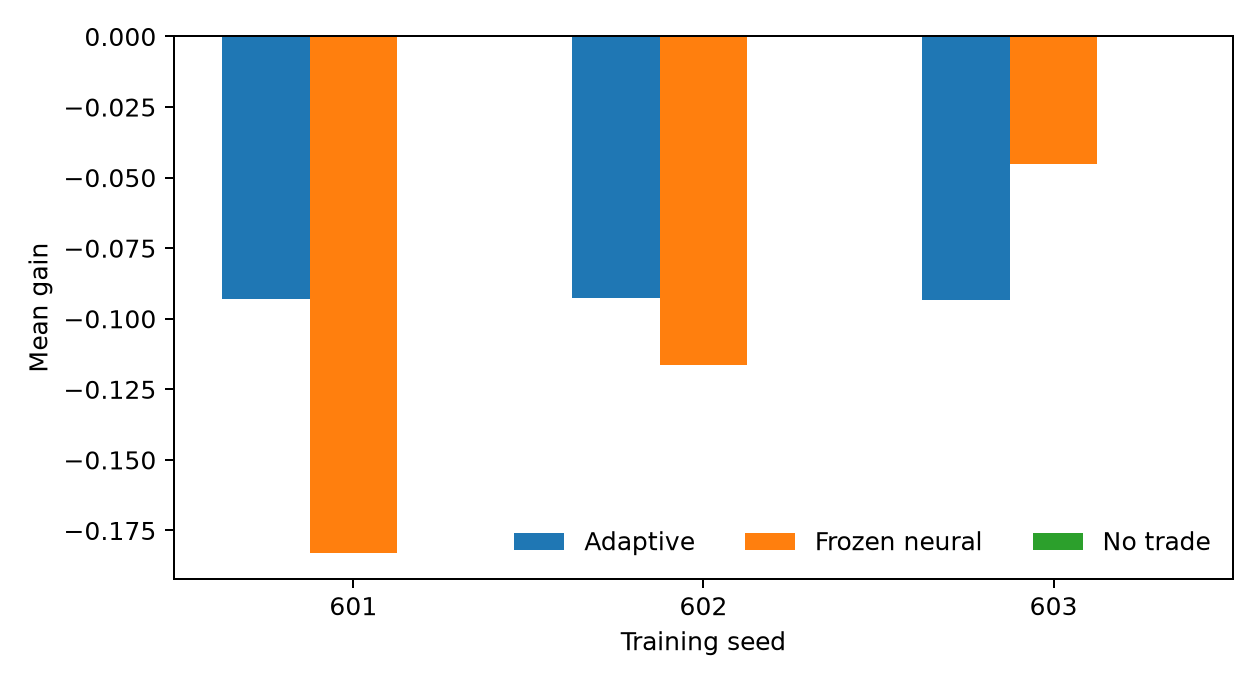
\includegraphics[width=0.86\linewidth]{next_stage_agent_gains.png}
\caption{Held-out paired gains by training seed. The no-trade rule has no
transaction loss in this environment; that is a baseline, not a profitable
strategy claim.}
\end{figure}

\begin{table}[t]
\centering\small
\caption{Observation diagnostics. Coverage, decisiveness, wrong-confidence,
and unresolved fractions are separate metrics.}
\ObservationResultsTable
\end{table}

The exact independent condition behaves as expected under this simulation. Once
measurement noise, dependence, and a smaller budget are combined, the
constrained condition has 0.790 coverage and 0.075 wrong-confident labels, while
0.905 of replicates remain unresolved at the declared decision threshold. The
result is a limitation of the implemented procedure, not evidence for a
universal impossibility theorem.

\begin{figure}[t]
\centering
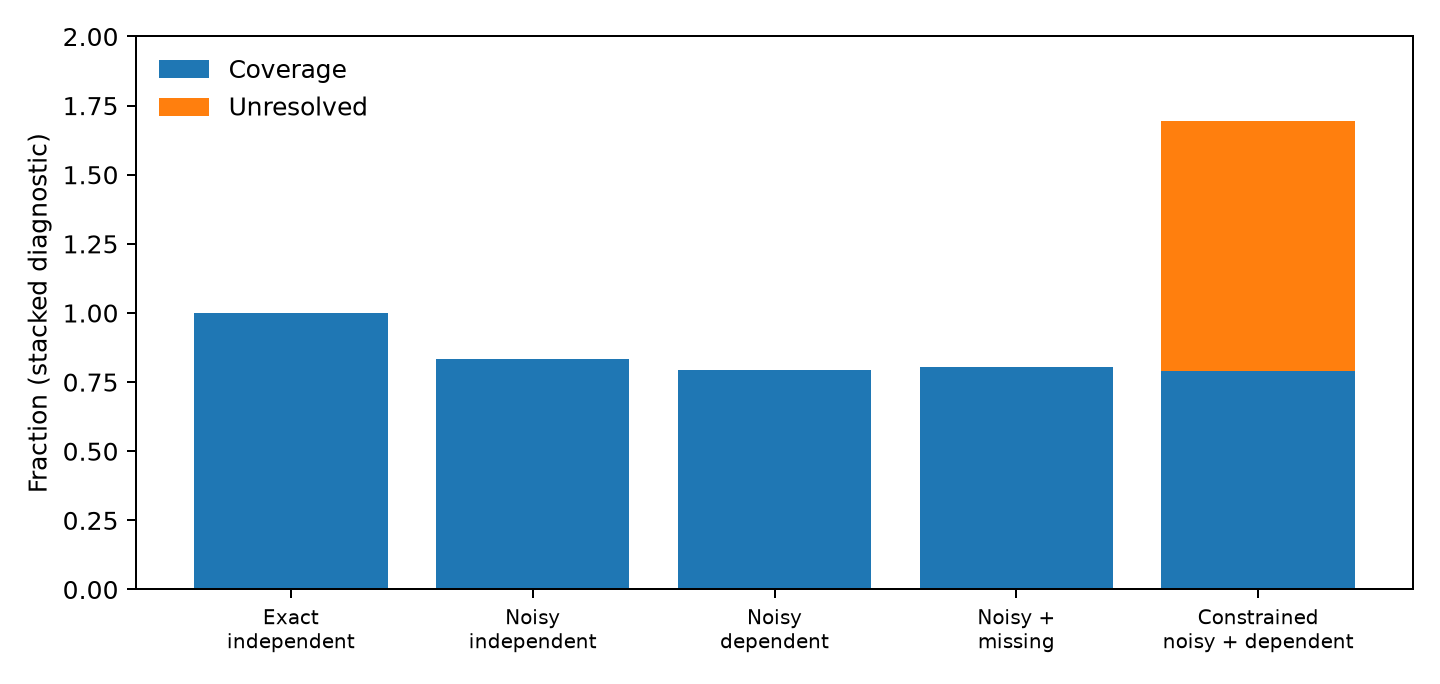
\includegraphics[width=0.90\linewidth]{next_stage_observation_diagnostics.png}
\caption{Observation coverage and unresolved diagnostics. The stacked display
is descriptive; the two fractions are not additive evidence of a probability
model.}
\end{figure}

\section{Operational-risk and intervention study}

The operational event is any nonterminal outcome: halt, default, margin breach,
or drawdown halt. A normal terminal settlement is not an event. The difficult
regime uses 50 units of initial cash, maximum order and inventory 1, volatility
0.02, impact 0.30, fee rate 0.002, margin rate 0.40, maintenance margin 0.10,
and drawdown limit 0.05. The three interventions were fixed before running 256
paired held-out tapes: no intervention, a 50\% order throttle, and inventory-
triggered liquidation.

\begin{table}[t]
\centering\small
\caption{Synthetic operational interventions.}
\InterventionResultsTable
\end{table}

The throttle lowers the local event rate and mean drawdown in this declared
single-account environment. Because there is no external dealer or second
account, the experiment cannot test loss shifting. Therefore it supports only a
conditional synthetic result, not an operational safety recommendation.

\begin{figure}[t]
\centering
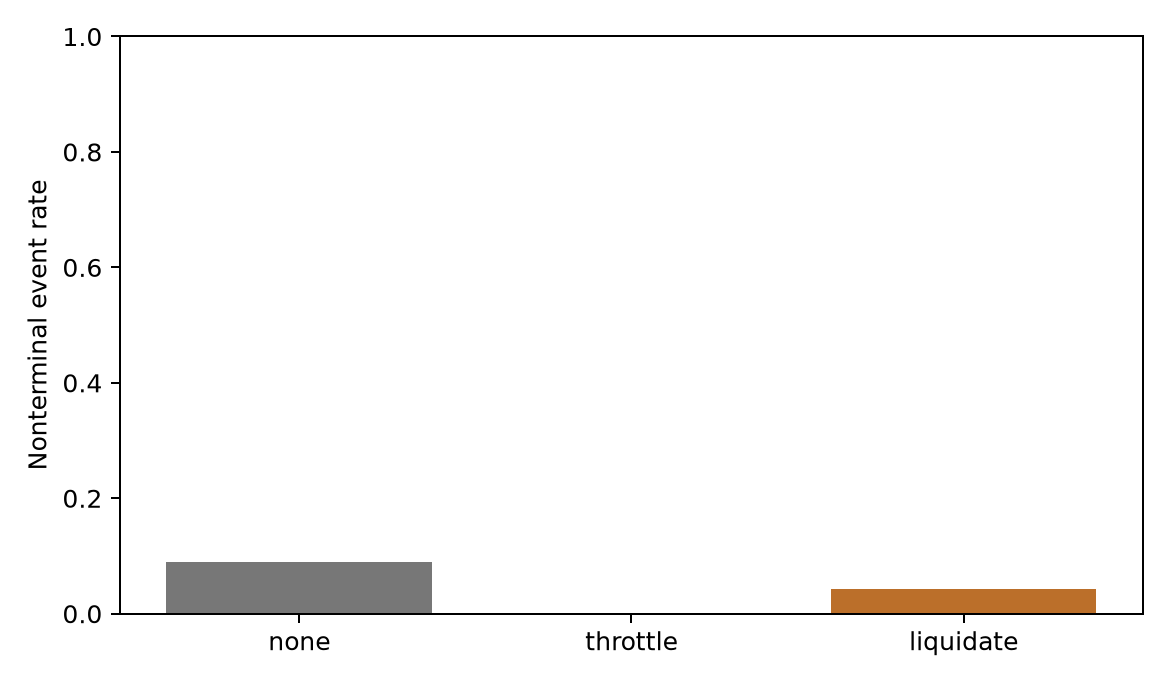
\includegraphics[width=0.76\linewidth]{next_stage_intervention_events.png}
\caption{Nonterminal event rates under the three fixed interventions.}
\end{figure}

\section{Public-data transfer boundary}

We load three public Binance monthly kline archives: BTCUSDT one-minute,
ETHUSDT one-hour, and SOLUSDT one-hour data from January 2025. The split is
chronological 60\% training, 20\% validation, and 20\% test. The resulting
descriptive counts are shown below.

\begin{table}[t]
\centering\small
\caption{Public OHLCV pilot split.}
\CalibrationResultsTable
\end{table}

These archives do not contain historical level-2 queue state, cancellations,
order priority, or enough information to validate partial-fill probabilities.
Consequently they do not establish a calibrated exchange replay environment.
WP13 remains externally blocked until authorized order-book data and a held-out
calibration succeed.

\section{Relation to the frozen release and failure cases}

The original release's internal tests and algebra checks remain the baseline;
they do not become external replication by being rerun. The next-stage package
preserves the following adverse findings: stronger full-horizon baselines can
outperform summary procedures, high-noise errors remain, omitted slow states
and false rate floors can produce false-stable labels, endpoint diversity is
not uniformly beneficial, and binding constraints can cause halts despite
local signal stability. The new results add a trained-policy null result and a
constrained observation failure mode.

\section{What is established}

Within the declared synthetic environment and seeds, the trained neural policy
does not clear the predeclared effect threshold against the adaptive
non-neural baseline. The evidence therefore supports a general adaptive-market
and measurement-limitation framing, not an AI-specific claim. The episode-block
benchmark demonstrates how noisy/dependent observations can lower coverage and
increase unresolved or wrong-confident decisions under a finite budget. The
intervention experiment demonstrates one conditional synthetic mechanism by
which execution throttling reduces local event rates.

\section{Limitations and open gates}

There is no independent external replication report, no authenticated
deployment/runtime attestation, no full historical order-book calibration, no
external operational validation, and no independent novelty, authorship,
ethics, or publication review. The trained policy is small and synthetic; its
failure to show an advantage is not evidence that all AI systems lack one.
No live trading, market perturbation, paid data, or unauthorized access was
used. The paper is internally reproducible at the declared level but is not
presented as publication-complete or safety-validated.

\section{Data and code availability}

The frozen release remains under \codelink{paper/} and \codelink{studies/}.
Run the new local confirmation package with:

\begin{verbatim}
python3.11 -m pytest -q studies/next_stage_validation/tests
python3.11 studies/next_stage_validation/scripts/run_all.py \
  --output studies/next_stage_validation/results --episodes 128
python3.11 studies/next_stage_validation/scripts/run_interventions.py \
  --output studies/next_stage_validation/results --episodes 256
python3.11 studies/next_stage_validation/scripts/run_observation_benchmark.py \
  --output studies/next_stage_validation/results --replicates 200
python3.11 studies/next_stage_validation/scripts/analyze_results.py
python3.11 studies/next_stage_validation/scripts/render_paper_artifacts.py
\end{verbatim}

The public-data acquisition manifest and checksums are in
\url{research_extension/data/acquisition_manifest.json}. Generated
results are versioned separately from the original master checksum manifest.

\section*{Contribution and review status}

The contribution record, AI-use disclosure, permissions, independent review,
and venue-specific rights are not finalized in this artifact. This section is
intentionally explicit so that a generated PDF is not mistaken for a completed
publication process.

\end{document}
